\chapter{Testautomatisierung}
\label{sec:testautomatisierung}
In Kapitel \ref{sec:testautoGrundlagen} wurde der Begriff Testautomatisierung bereits eingeführt. Die darin gewählte Definition hat gezeigt, dass man unter Testautomatisierung weit mehr versteht, als das automatisierte ausführen von Testfällen auch wenn das der wohl am weitesten verbreiteten Bereich der Automatisierung ist.
Testautomatisierung ist in allen Bereichen des Entwicklungs- bzw. Testprozesses möglich.
\glqq Das Spektrum umfasst alle Tätigkeiten zur überprüfung der Softwarequalität im Entwicklungsprozess, in den unterschiedlichen Entwicklungsphasen und Teststufen so wie die entsprechenden Aktivitäten von Entwicklern, Testern, Analytikern oder auch der in die Entwicklung eingebundenen Anwender. Die Grenzen der Automatisierung liegen darin, dass diese nur die manuellen Tätigkeiten eines Testers übernehmen kann, nicht aber die intellektuelle, krative und intuitive Dimension dieser Rolle.\grqq\ \cite[S.7]{seidl_basiswissen_2012}
Diese intellektuelle Dimension ist vor allem in den frühen Phasen des Testprozesses gefordert. Diese Phasen sind maßgeblich für die Spätere Qualität der einzelnen Testfälle. Testautomatisierung wird daher nie die arbeiten eines guten Testanalysten voll ersetzen können. Um so weiter der Testprozess voranschreitet, um so p
raktischer werden auch die zu erledigenden Aufgaben. Das Potential für eine Automatisierung steigt.
Fewster et al. stellen diesen Zusammenhang in einer Grafik bildlich dar. \cite[vgl. S.18]{fewster_software_1999} Abbildung \ref{fig:intellektuellVsPraktisch} greift diese Darstellung auf und passt sie auf den in Kapitel \ref{sec:testprozess} vorgestellten Testprozess an. Die verschiedenen Möglichkeiten der Testautomatisierung werden in Kapitel \ref{sec:bereiche_der_estautomatisierung} geklärt. Zunächst soll jedoch die Frage beantwortet werden warum eine Automatisierung von Testfällen überhaupt Sinn macht.

\begin{figure}[htb]
  \centering  
  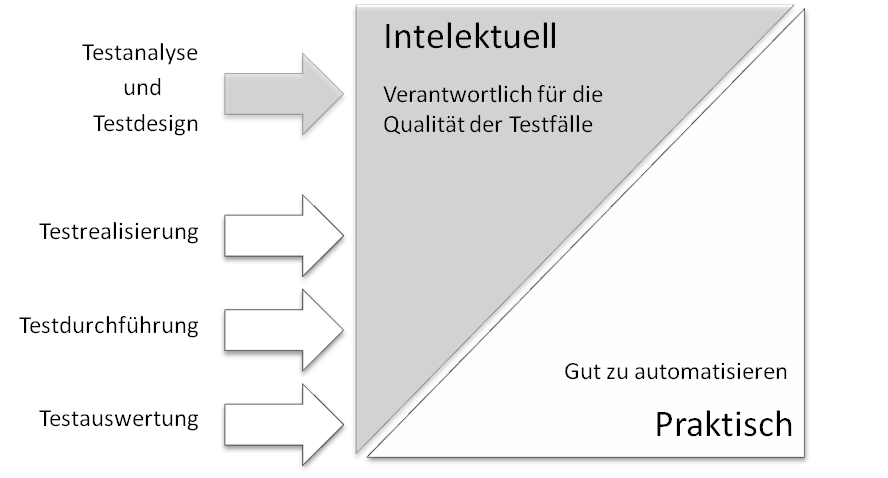
\includegraphics[scale=1]{img/intelektuellVsPraktisch.png}\\
  \footnotesize\sffamily\textbf{Quelle:} \cite[vgl. S.18]{fewster_software_1999}
  \caption{Grenzen und Möglichkeiten der Testautomatisierung}
  \label{fig:intellektuellVsPraktisch}
\end{figure}

\section{Warum Testautomatisierung}
\label{sec:warum_testautomatisierung}

Richtig durchgeführt kann Testautomatisierung eine Reihe von Vorteilen bringen. Dustin et al. stellen drei bedeutende Vorteile der Testautomatisierung fest. \cite[S.44 ff.]{dustin_software_2001}
\begin{itemize}
\item[1.] Erstellung eines zuverlässigen Systems
\item[2.] Verbesserung der Testqualität und Testtiefe
\item[3.] Verringerung des Testaufwands und Reduzierung des Zeitplans
\end{itemize}

Diese Vorteile stehen in enger Abhängigkeit zueinander. Eine Verringerung des Testaufwands für einzelne Tests schafft mehr Zeit die in bessere und breiter angelegte Tests investiert werden kann. Neben der direkten Beeinflussung führt Testautomatisierung also zusätzlich auch indirekt zu einer höhere Testqualität und Testtiefe. Diese bedingt dann wiederum dass mehr Fehler im System aufgedeckt werde können. So kann eine höhere Qualität des Endproduktes erreicht werden die sich in einem zuverlässigeren System zeigt.

In der Literatur gibt es zahlreiche Listen von Vorteilen der Testautomatisierung die bereits sehr fein gegliedert sind. \cite{fewster_software_1999} \cite{thaller_software-test_2002}
Gleicht man diese Vorteile mit den von Dustin et al. gewählten Oberpunkten ab zeigt sich, dass vor allem die Punkte 2 und 3 also Qualität und Effezienz gut durch diese repräsentiert werden. Sie lassen sich leicht mit den Vorteilen anderer Autoren unterfüttern. Die Erstellung eines zuverlässigen Systems ist hingegen nur schwer direkt zu beeinflussen. In der Regel wird dieser Punkt wie oben beschrieben indirekt beeinflusst.
Im folgenden wird daher dieser Punkt nicht weiter betrachtet. Die feiner gegliederten Vorteile wie sie Fewster et al. beschreiben werden Verbesserung der Testqualität und Testtiefe so wie der Verringerung des Testaufwands und Reduzierung des Zeitplans zugeordnet.


Während das zuverlässige System eher eine Folge aus höherer Effizienz und Qualität im Testen sind, können der Qualitätsgewinn und die Effizienzsteigerung durch feinere Vorteile unterfüttert werden.



\section{Möglichkeiten der Testautomatisierung im Testprozess}
\label{sec:bereiche_der_estautomatisierung}
Einteilung nach testprozess nicht perfekt. Dahre eine einteilung die der automatisierung besser passt:
A Search-Based Approach for Cost-Effective Software Test Automation Decision Support and an Industrial Case Study

\subsection{Testdesign}
\label{subsec:testdesign}


\subsection{Testcodeerstellung}
\label{subsec:testcodeerstellung}
c and r

\subsection{Testdurchführung}
\label{subsec:testdurchführung}


\subsection{Testauswertung}
\label{subsec:testauswertung}



\section{Schnittstellen der Testautomatisierung zum System}
\label{sec:schnittstellen_der_testautomatisierung_zum_syste}

Jeder testfall muss in irgendeiner weise mit dem zu testenden objekt interagieren.
Analog zu manuellen tests gibt es hierfür verschiedene möglichkeiten.
\subsection{API}
\subsubsection{JUnit}
\label{sec:junit}

\subsection{GUI}
Web
